%!TEX root = ../document.tex
\chapter{Project Organizational Structure}

\section{Project organizational chart}

The Flying Vehicle Design and Production project team consists of a project steering committee, a customer service team, a project manager, a functional team, and a technical team. The project was initiated by the Project Steering Committee, which is also the main decision maker and strategy maker for the project. All project matters are coordinated and managed by the project team. The project team will consist of full-time project managers, technicians, and business owners and experts in key functional areas.In addition, the project team will include technical and functional consultants from the client side.

\begin{figure}[!htb]
\centering
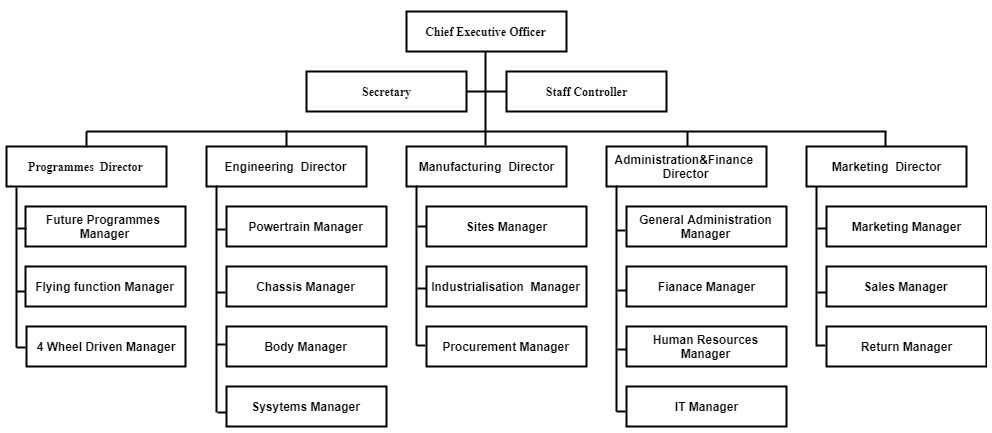
\includegraphics[width=15cm]{pic/structure.jpg}
\end{figure}

\section{Responsibility}

The work of this project is completed by a project team composed of Ethane Autoplane Co.Ltd. and the client side, which means that the two parties form a common working group in the project to complete each project task. The main consideration of this arrangement is to ensure that the design and manufacturing of the flight and the car meet the customer's requirements during the project, and when necessary, communicate with the customer about the design details of the flying car, and coordinate the design between the designer and the customer. Only in this way can the order of the design and manufacturing of the flying car be guaranteed.

Specifically, the division of labor and responsibilities of Ethane Autoplane Co.Ltd and the client are:

\subsection{Project management team responsibilities}

\renewcommand\arraystretch{1.2}
\begin{table}[!htb]
\centering
\footnotesize
\begin{tabular}[b]{|p{2cm}<{\raggedright}|p{2cm}<{\raggedright}|p{10.5cm}<{\raggedright}|}
\hline
Role & Personnel & Description \\
\hline
Steering Committee Member/Project Director & Related personnel & 
\ding{212} Support and monitor project actions;\par
\ding{212} Review/approve the project plan with the leader;\par
\ding{212} Review/modify/approve the guidelines proposed by the project team with the leadership;\par
\ding{212} Provide advanced project management guidance and assistance;\par
\ding{212} Evaluate the design and manufacture of products to ensure that quality meets certain requirements, timely delivery and cost control. \\
\hline
project manager &	Related personnel	&	
\ding{212} Provide project management services;\par
\ding{212} Coordinate the allocation of resources among all project teams;\par
\ding{212} Develop, monitor and implement project plans and related work schedules;\par
\ding{212} Organize project progress status meetings, prepare/release project communication/reports;\par
\ding{212} Monitor project progress, task completion, and resource allocation and benefits of the project;\par
\ding{212} Management issues to resolve progress; assign priorities and monitor the implementation of relevant corrective actions;\par
\ding{212} Manage the change control process;\par
\ding{212} Assist in defining change management needs;\par
\ding{212} Provide general advice or support on functional/technical matters. \\
\hline
Project supervision &	Related personnel &	Provide supervision, consulting and support for business, technology, management, etc. \\
\hline
\end{tabular}
\end{table}

\subsection{Product development team}

\renewcommand\arraystretch{1.2}
\begin{table}[H]
\centering
\footnotesize
\begin{tabular}[b]{|p{2cm}<{\raggedright}|p{2cm}<{\raggedright}|p{10.5cm}<{\raggedright}|}
\hline
Role & Personnel & Description \\
\hline
Development manager &	Related personnel	&	
\ding{212} Provide project management services;\par
\ding{212} Coordinate the allocation of resources among all project teams;\par
\ding{212} Develop, monitor and implement project plans and related work schedules;\par
\ding{212} Organize project progress status meetings, prepare/release project communication/reports;\par
\ding{212} Monitor project progress, task completion, and resource allocation and benefits of the project;\par
\ding{212} Management issues to resolve progress; assign priorities and monitor the implementation of relevant corrective actions;\par
\ding{212} Manage the change control process;\par
\ding{212} Assist in defining change management needs;\par
\ding{212} Provide general advice or support on functional/technical matters. \\
\hline
Functional engineer &	Related personnel	&	
\ding{212} Provide relevant knowledge to realize the function of flying vehicles;\par
\ding{212} Prepare a detailed implementation plan for the project task;\par
\ding{212} Business needs and variance analysis;\par
\ding{212} Provide guidance and advice for system design;\par
\ding{212} Guide and help define requirements and methods related to process and end-user training;\par
\ding{212} Lead system configuration, enablement and security work;\par
\ding{212} Auxiliary and participate in system testing strategies, planning and test execution;\par
\ding{212} Lead and find faults and problems found in integration testing;\par
\ding{212} Provide consulting services during the development of the end user process;\par
\ding{212} Provide consulting services related to end-user training materials and training implementation. \\
\hline
Technical engineer & Related personnel & 
\ding{212} Teaching knowledge related to the design and manufacture of flying vehicles;\par
\ding{212} Prepare an implementation plan for the technical project components;\par
\ding{212} Prepare indicators and estimates, participate in variance analysis, and assist with product design;\par
\ding{212} Responsible for the primary responsibility for custom development listed in the scope definition, or provide the functionality described in the project definition as needed;\par
\ding{212} Advice and assistance in the design of technical environment architectures and processes;\par
\ding{212} The leader found problems in the system test and user acceptance test. \\
\hline
\end{tabular}
\end{table}

\subsection{Project promotion team and coordination group}

The ultimate owner of a flying car product is not the project team, nor the manufacturing staff, but the entire staff of the project, including the leaders of all departments and all employees. So throughout the project, the involvement, input, and support of these people play a key role in the success of the entire project. It is therefore necessary to clarify the responsibilities of these people for the project.

\renewcommand\arraystretch{1.2}
\begin{table}[H]
\centering
\footnotesize
\begin{tabular}[b]{|p{2cm}<{\raggedright}|p{2cm}<{\raggedright}|p{10.5cm}<{\raggedright}|}
\hline
Role & Personnel & Description \\
\hline
Project promotion team member	& Related personnel	&	
\ding{212} Responsible for the promotion and promotion of flying car products;\par
\ding{212} Timely solve problems in the process of project implementation and communicate with the project team;\par
\ding{212} Responsible for organizing personnel to participate in end-user testing of the product;\par
\ding{212} Ensure that all employees in the department receive adequate product production design training;\par
\ding{212} After the product is successfully developed, ensure that all system-related manufacturing processes in the department are carried out according to the project design, for example, in accordance with the determined approval rules. \\
\hline
Project coordination team member & Related personnel & 
\ding{212} Cooperate with the project team and department leaders, coordinate the specific work carried out by the production and manufacturing system in the department, and serve as the working bridge between the project team and the department;\par
\ding{212} Responsible for collecting and collating data according to the requirements of the project team. After the data migration is completed, the project team is responsible for data verification;\par
\ding{212} Participate in end-user training as required by the project team;\par
\ding{212} Responsible for organizing employees of the department to participate in manufacturing system training;\par
\ding{212} Responsible for other communication and coordination work between the project team and the department. \\
\hline
\end{tabular}
\end{table}

\subsection{Other participants and groups of the project}

\renewcommand\arraystretch{1.2}
\begin{table}[H]
\centering
\footnotesize
\begin{tabular}[b]{|p{2cm}<{\raggedright}|p{2cm}<{\raggedright}|p{10.5cm}<{\raggedright}|}
\hline
Role & Personnel & Description \\
\hline
Key user & Related personnel & 
\ding{212} Representatively participate in project teams, user testing, and support group activities;\par
\ding{212} Experience the product and provide feedback.\\
\hline
User test group &	Related personnel &	
\ding{212} Representing the interests of business owners and end users in key actions;\par
\ding{212} Provide advice/assistance when the project makes decisions that affect the end user;\par
\ding{212} Is a decision maker who decides whether a product can be accepted;\par
\ding{212} Provide feedback.\\
\hline
Training/ Process / Test Group & Related personnel & 
\ding{212} Representing the interests of business owners and end users in key actions;\par
\ding{212} Responsible for the development and execution of strategies and plans related to end-user training business process improvement and end-user testing.\\
\hline
\end{tabular}
\end{table}

\section{Responsibility matrix}

\ding{108} Be responsible

\ding{70} Participate/guide

\ding{71} Supervise

\newcommand{\tabincell}[2]{\begin{tabular}{@{}#1@{}}#2\end{tabular}}
\renewcommand\arraystretch{1.2}
\begin{table}[H]
\centering
\footnotesize
\begin{tabular}[b]{|p{2cm}<{\raggedright}|p{2cm}<{\raggedright}|p{3cm}<{\raggedright}|p{1cm}<{\raggedright}|p{1cm}<{\raggedright}|p{1cm}<{\raggedright}|p{1cm}<{\raggedright}|p{1cm}<{\raggedright}|}
\hline
\multicolumn{2}{|l|}{ \multirow{2}{*}{Project task} } & \multirow{2}{*}{Key deliverable} & \multicolumn{4}{|l|}{Party B} & Party A \\
\cline{4-8}
\multicolumn{2}{|l|}{} &  & Project manager &	Project supervision &	Develop- ment team &	business manager & Project manager \\  
\hline
\multirow{5}{*}{\tabincell{l}{Project \\ begining}} & Signing the project charter	& Project charter & \ding{108} &  &  & \ding{70} & \ding{108} \\
\cline{2-8}
                                  & Project implementation plan	& Project outline plan 	& \ding{108} & \ding{70} & \ding{70} & \ding{70} & \ding{71} \\
\cline{2-8}                             
                                  & Hold a kickoff meeting &	Meeting record	& \ding{108} & \ding{70} & \ding{70} &\ding{70}  & \ding{108} \\
\hline
\multirow{5}{*}{\tabincell{l}{Project \\ product \\ planning}} & Product design and development &	Product design document	& \ding{108}  & \ding{70} & \ding{108}  &  & \ding{108} \\
\cline{2-8}
                                  & Product testing &	Product testing document	& \ding{70} & \ding{70} & \ding{70} &  & \ding{71} \\
\hline
\multirow{5}{*}{\tabincell{l}{ Project \\ testing } } & Safety test	& testing report & \ding{70} & \ding{71} & \ding{108} &  & \ding{71} \\
\cline{2-8}
                                  & Performance Testing	& testing report 	& \ding{70} & \ding{71} & \ding{108} &  & \ding{71} \\
\cline{2-8}                             
                                  & User experience test &	testing report	& \ding{70} & \ding{71} & \ding{108} &  & \ding{71}\\
\hline
\multirow{5}{*}{\tabincell{l}{ Project \\ closing } } & Technical handove	& Project operation and maintenance plan & \ding{108} & \ding{71} & \ding{108} &  & \ding{70} \\
\cline{2-8}
                                  & Project Acceptance	& Project acceptance report 	& \ding{108} & \ding{71} & \ding{108} & \ding{70} &\ding{108}  \\
\hline
\multirow{5}{*}{\tabincell{l}{ Project \\ management } } & Weekly meeting	& Weekly work summary and plan & \ding{108} & \ding{71} & \ding{108} & \ding{70} & \ding{108} \\
\cline{2-8}
                                  & Project event management	& memorandum 	& \ding{108} & \ding{71} & \ding{108} & \ding{70} & \ding{108} \\
\cline{2-8}                             
                                  & Demand change &	Request for Change Request Form	& \ding{108} & \ding{71} & \ding{108} & \ding{70} & \ding{108}\\
\hline
\end{tabular}
\end{table}
